\begin{frame}{Polymorphism}
    \begin{block}{Definition}
        Polymorphism is the ability of a function to behave ``correctly'' on different data types.
    \end{block}
    \begin{block}{Properties}
        \begin{itemize}
            \item Polymorphism is a key concept in functional programming.
            \item Polymorphism allows for the definition of functions that can be applied to a range of data types.
        \end{itemize}
    \end{block}
\end{frame}
\begin{frame}
    \centering
    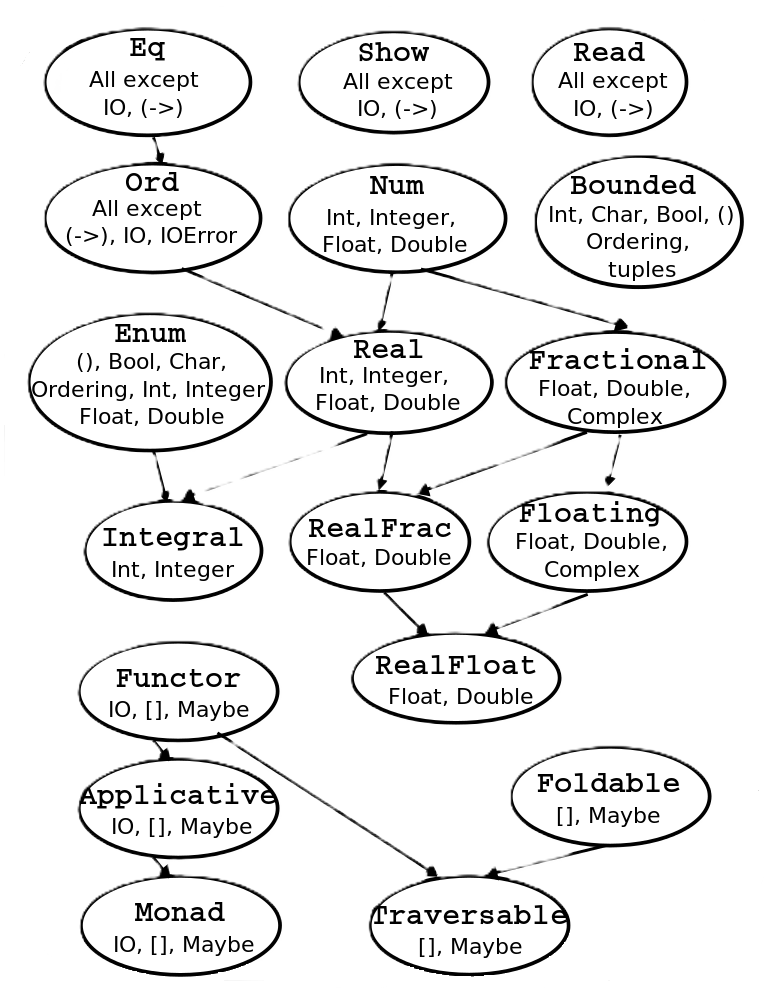
\includegraphics[height=.8\textheight]{resources/figures/lecture_01/typing/Base_classes_hierarchy.png}
    {\tiny \url{https://en.wikibooks.org/wiki/Haskell/Classes_and_types}}
\end{frame}